\documentclass{beamer}
\usepackage[utf8]{inputenc}
\usepackage{graphicx}
\usepackage{url}

\author[Sowmya Vajjala]{Instructor: Sowmya Vajjala}


\title[LING 120]{LING 120: \\ Language and Computers}
\subtitle{Semester: Fall '17}

\date{13 November 2017}

\institute{Iowa State University, USA}

%%%%%%%%%%%%%%%%%%%%%%%%%%%

\begin{document}

\begin{frame}\titlepage
\end{frame}

\begin{frame}
\frametitle{Outline}
\begin{itemize}
\item General Announcements
\item Discussion about previous exercise
\item Plan for this week: 
\begin{itemize}
\item Machine Translation: introduction (today and wednesday)
\item Friday: General discussion about different applications, impact of these on our life etc. 
\item How does Machine Translation work? (after the break)
\end{itemize}
\item Exercise about Machine Translation
\end{itemize}
\end{frame}

\begin{frame}
\frametitle{}
\Large General Announcements
\end{frame}

\begin{frame}
\frametitle{General Stuff}
\begin{itemize}
\item \textbf{Reminder: }Assignment 6 due this week!
\item Revision topics: no one posted anything
\item But I was reading about representing Sign Language and Braille on computer over the weekend - may be I will try to know more and talk about this after the break.
\end{itemize}
\end{frame}

\begin{frame}
\frametitle{Grade improvement: oral exam timings}
People wanting grade improvement, choose one of the following timings and get back:
\begin{itemize}
\item 4th December: 1-2 pm, 5-5:30 pm. 6th December: 1-2pm, 5-5:30 pm. 8th December: 1-2 pm.
\item Choose a time (actual oral exam will only take 15 min), choose any 3 topics from the course, and send me an email.
\item Show up at the time you promised to come, and I will pick one (or two) of the three topics and ask questions.
\item Maximum improvement: 5\% (I am flexible if you do extraordinarily well)
\end{itemize}
\end{frame}

\begin{frame}
\frametitle{Final Exam: Recap of description}
\begin{itemize}
\item Carries: 20\% of your grade, and involves writing 2 short essays. 
\item Has to be submitted in three parts:
\begin{enumerate}
\item Write a part of the assignment (one question) and submit by 2nd December - 5\%
\item Do an in-class peer review of one of your classmate's work (6th December) - 5\% - if you don't come to class, you don't get graded for this part.
\item Final submission (of both the questions) - 10\%
\end{enumerate}
\item Exact details about word limits, how to submit and list of topics for questions are on Canvas. 
\end{itemize}
\end{frame}

\begin{frame}
\frametitle{Final Exam- Questions?}
\begin{itemize}
\item I am hoping you read through the requirements and expectations
\item I am also hoping you now know the deadlines
\item Any questions on finals?
\end{itemize}
\end{frame}

\begin{frame}
\frametitle{}
\Large Discussion of Last Class Exercise
\end{frame}

\begin{frame}
\frametitle{Attendance Exercise From Last Class}
Running on MT - \url{http://nacloweb.org/resources/problems/2011/A.pdf} \\
\medskip
Solution: 
\begin{itemize}
\item Looking for words that seem out of place
\item Thinking about synonyms of those words that fit in the context.
\item Full list: \url{http://nacloweb.org/resources/problems/2011/naclo11r1_sol.pdf}
\end{itemize}
\end{frame}

\begin{frame}
\frametitle{}
Nellie on Speech-Speech Translation in Skype
\end{frame}

\begin{frame}
\frametitle{}
\Large Intro to Machine Translation
\end{frame}

\begin{frame}
\frametitle{Questions, questions, questions!}
\begin{itemize}
\item Is translation easy for humans? \pause
\item What in your idea should machine translation do? \pause
\item For humans:
\begin{itemize}
\item What is possibly easy to translate? \pause
\item What is possibly difficult to translate? \pause
\item What do you think is impossible to translate? \pause
\end{itemize}
\item What do you think is the case for machines? \pause
\item What are the applications of machine translation? \pause
\item How do we evaluate human translation? \pause
\item How do we evaluate machine translation? 
\end{itemize}
\end{frame}

\begin{frame}
\frametitle{Let us talk about Human Translation first}
Can 2--3 people who can speak/read/write in another language come forward and translate the following sentence:

\medskip

Why do we need machine translation? 

\end{frame}


\begin{frame}
\frametitle{Machine Translation today - Example 1}
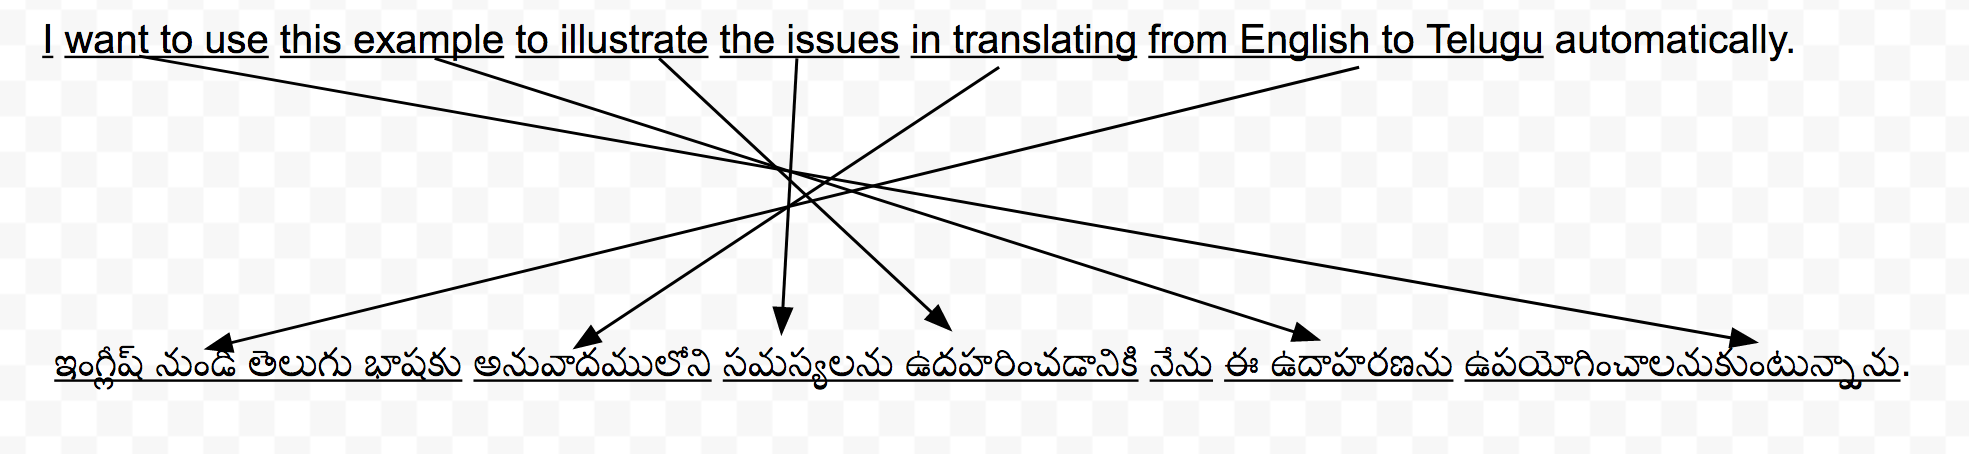
\includegraphics[height=10cm,width=1.1\textwidth,keepaspectratio]{MTEngTelExample1}
\end{frame}

\begin{frame}
\frametitle{Machine Translation today- Example 2}
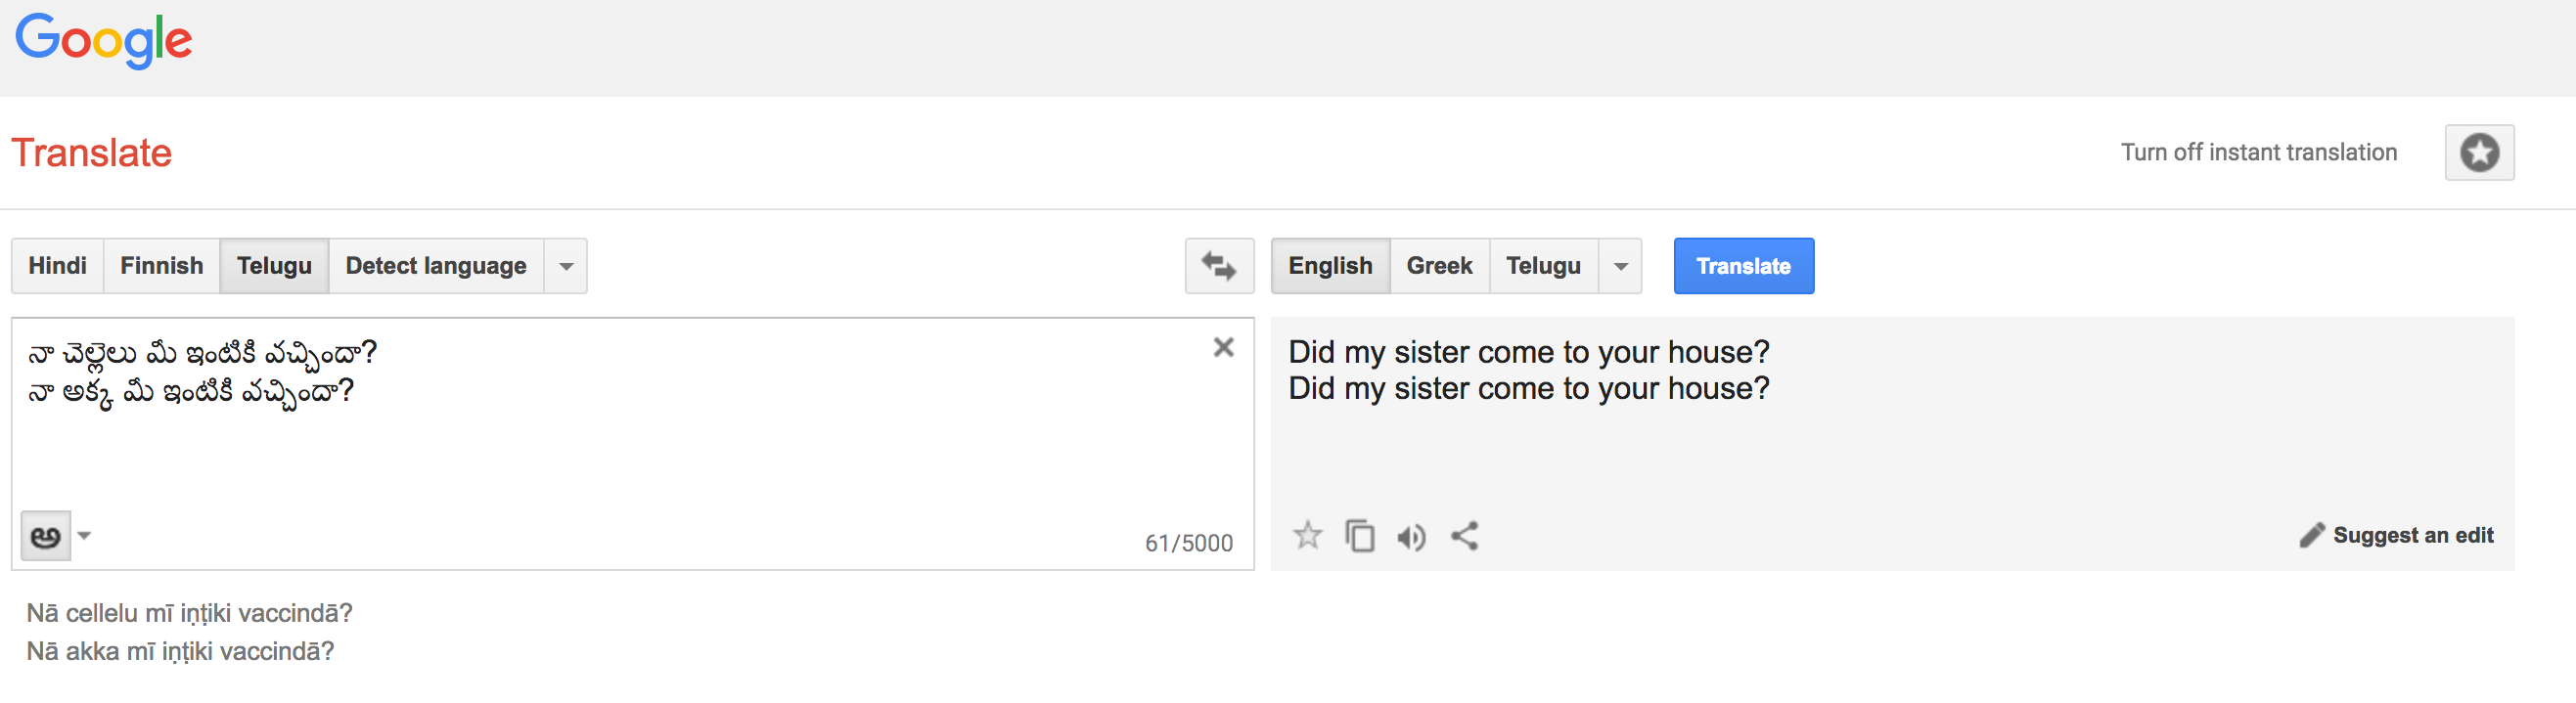
\includegraphics[height=10cm,width=1.1\textwidth,keepaspectratio]{chelleluakka}
\end{frame}

\begin{frame}
\frametitle{Machine Translation today- Example 3}
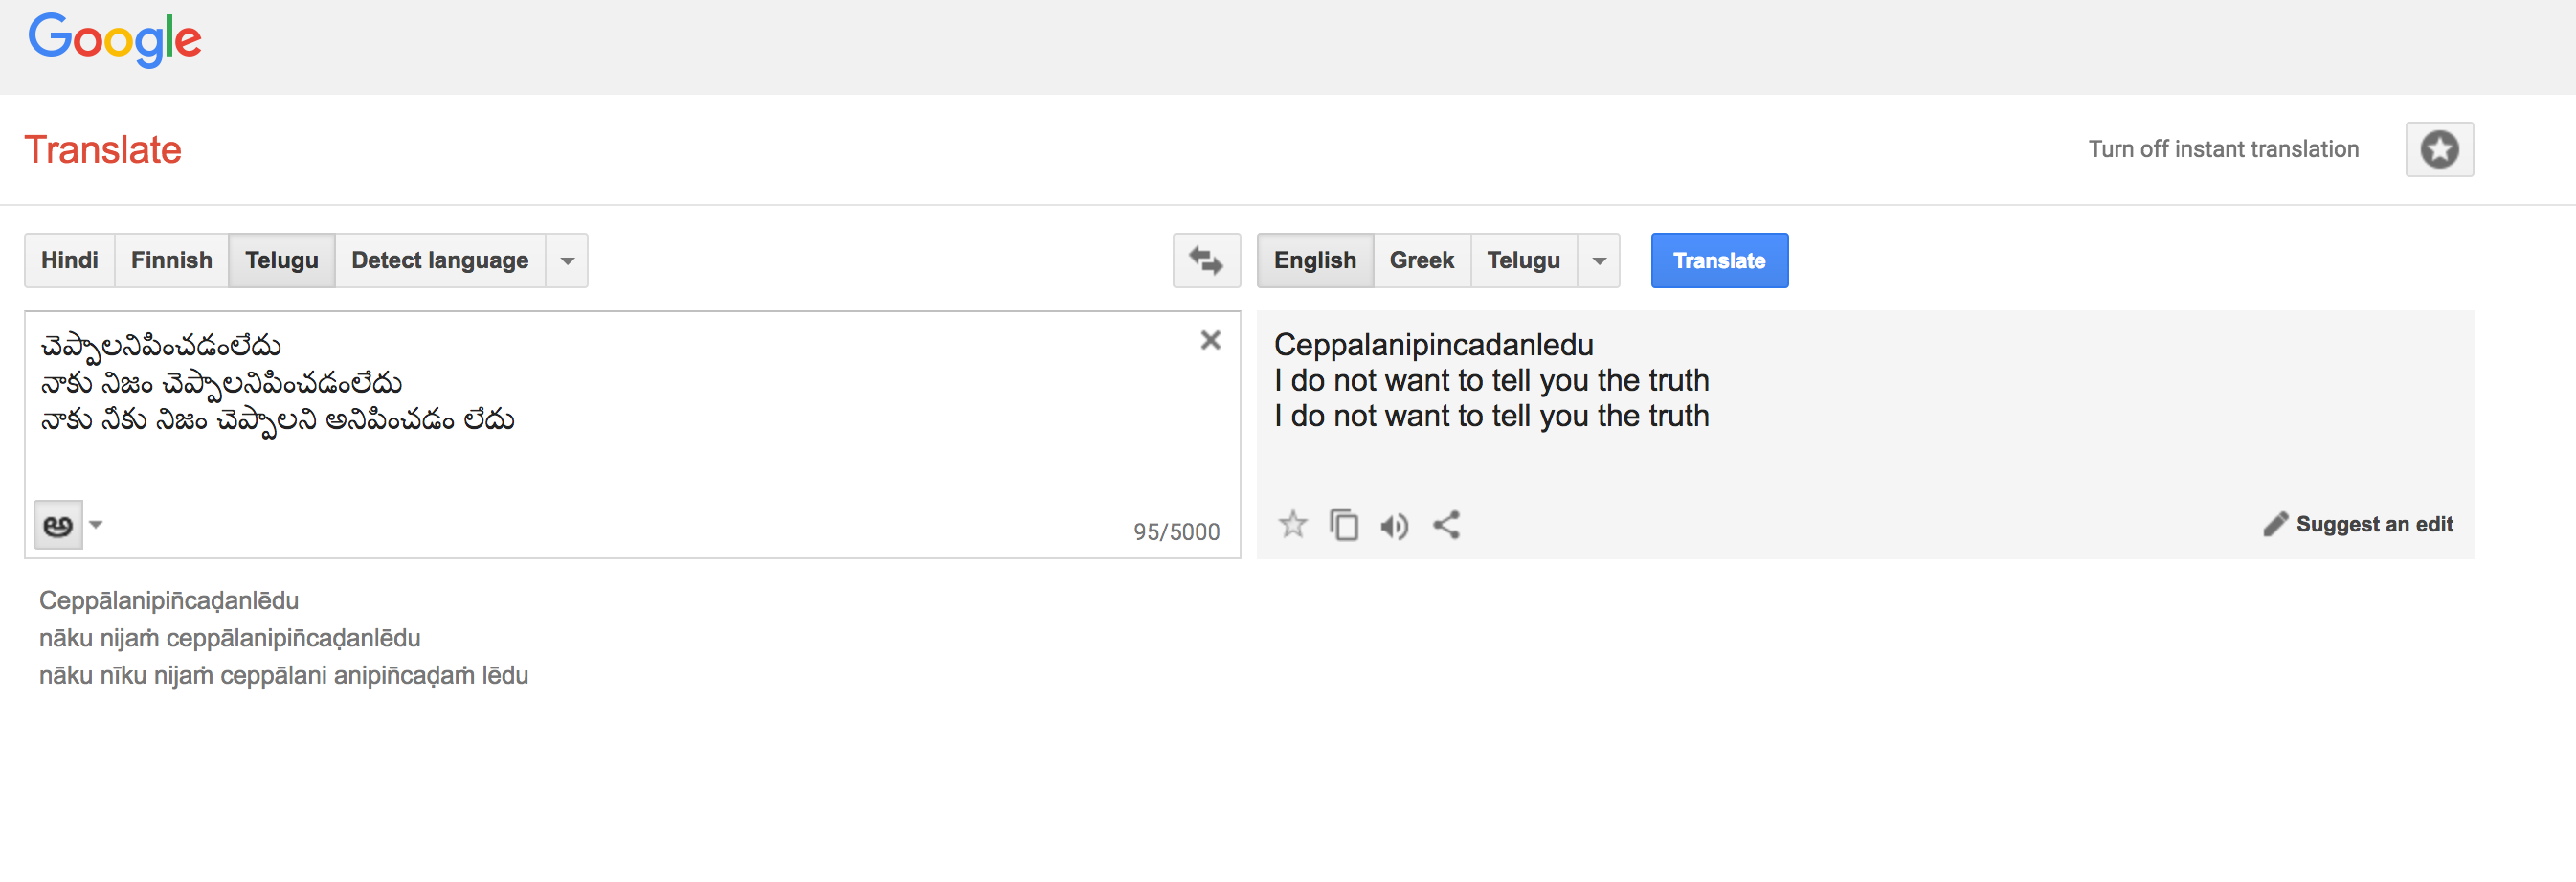
\includegraphics[height=10cm,width=1.1\textwidth,keepaspectratio]{MTEngTelExample2}
\end{frame}

\begin{frame}
\frametitle{So, what are the issues?}
\begin{itemize}
\item From last class, we also know: Each word can have multiple meanings, so mapping words one-one between languages is not possible.
\item From today's examples, we know there are several other issues such as:
\begin{itemize}
\item How words are formed between languages
\item What is the order of words
\item Words that don't seem to translate
\item Words that seem to come up in translation that do not exist in original
\item Issues such as: articles don't exist in Telugu, but they do in English. Kinship words are more fine grained in Telugu than English etc. 
\end{itemize}
\end{itemize}
\end{frame}

\begin{frame}
\frametitle{Other Issues}
\begin{itemize}
\item Stylistic and cultural differences - which can make even manual translation difficult
\item Metaphor is even difficult - same metaphors need not exist in both languages
\item Poetry with rhyme - what if those words don't rhyme in Target language?
\end{itemize}
\end{frame}

\begin{frame}
\frametitle{Different Scenarios for Machine Translation}
\begin{itemize}
\item Tasks where rough translation is adequate (e.g., doing a web search)
\item Tasks where a human post-editor is used (e.g., computer aided human translation, to reduce effort for human translators, in scenarios like creating multi-lingual interfaces to Windows, Facebook etc)
\item Tasks within a restricted domain, which need high quality translation (e.g., Weather forecasting)
\end{itemize}
\end{frame}

\begin{frame}
\frametitle{Today's Attendance Exercise}
In this course so far, where is the idea of n-grams useful among the topics we discussed? Do you think they are useful in Machine Translation too? 
\\ Just an FYI: our main topics were - text and speech input, spelling and grammar correction, tutoring systems, search, text classification, dialog systems, speech recognition and synthesis. 
\end{frame}

\end{document}
